\documentclass[a4paper,landscape]{article}


\usepackage{tikz}
 \usetikzlibrary{arrows}
\usetikzlibrary{fit,positioning}



\begin{document}

%\centering
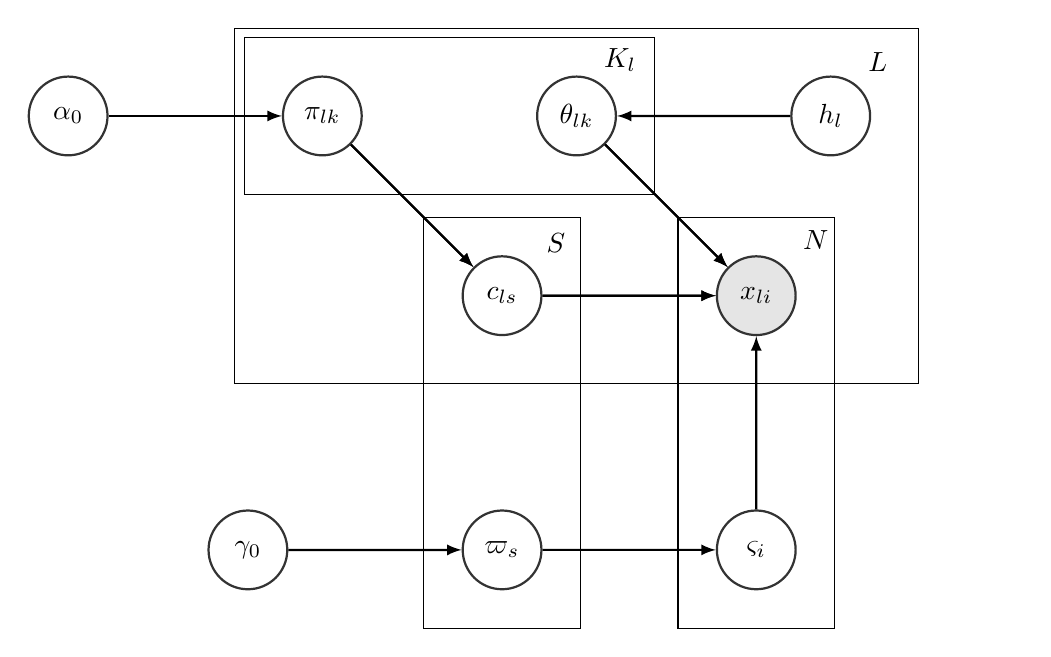
\begin{tikzpicture}[scale=.7, auto,>=latex']
\tikzstyle{main}=[circle, minimum size = 10mm, thick, draw =black!80, node distance = 22mm]
\tikzstyle{connect}=[-latex, thick]
\tikzstyle{box}=[rectangle, draw=black!100]
 \node[main] (pi) {$\pi_{lk}$ };
 \node[main] (a) [left=of pi] {$\alpha_0$ };
 \node[main] (ci) [below right=of pi] {$c_{ls}$};
 \node[main, fill = black!10] (xi) [right=of ci] {$x_{li}$};
 \node[main] (theta) [above left=of xi] {$\theta_{lk}$};
 \node[main] (varsig) [below=of xi] {$\varsigma_i$};
 \node[main] (varpi) [left=of varsig] {$\varpi_s$};
 \node[main] (gamma0) [left=of varpi] {$\gamma_0$};
 \node[main] (hl) [right=of theta] {$h_l$};
 \path (pi) edge [connect] (ci)
		(ci) edge [connect] (xi)
		(theta) edge [connect] (xi)
		(a) edge [connect] (pi);
 \node[rectangle, inner sep=-0.5mm, fit= (varsig) (xi),label=above right:$N$, xshift=0mm, yshift=16mm] {};
 \node[rectangle, inner sep=4.8mm,draw=black!100, fit= (varsig) (xi)] {};
 \node[rectangle, inner sep=-0.8mm, fit= (theta) (pi),label=above right:$K_l$, xshift=14mm] {};
 \node[rectangle, inner sep=4.8mm, draw=black! 100, fit= (theta)(pi)] {};
\node[rectangle, inner sep=4.8mm, draw=black! 100, fit= (theta)(pi)] {};
 \node[rectangle, inner sep=-0.8mm, fit= (ci) (varpi),label=above right:$S$, xshift=0mm, yshift=16mm] {};
 \node[rectangle, inner sep=4.8mm, draw=black! 100, fit= (ci) (varpi)] {};
 \node[rectangle, inner sep=-0.8mm, fit= (ci) (xi) (theta) (pi) (hl),label=above right:$L$, xshift=20mm] {};
 \node[rectangle, inner sep=6.0mm, draw=black! 100, fit= (ci) (xi) (theta) (pi) (hl)] {};

 \path (pi) edge [connect] (ci)
		(ci) edge [connect] (xi)
		(theta) edge [connect] (xi)
		(hl) edge [connect] (theta)
		(varsig) edge [connect] (xi)
		(varpi) edge [connect] (varsig)
		(gamma0) edge [connect] (varpi);
\end{tikzpicture}

\end{document}